\documentclass[11pt,a4paper]{article}

\usepackage[T1]{fontenc}
\usepackage{lmodern}
\usepackage{microtype}
\usepackage[a4paper,margin=2.5cm]{geometry}
\usepackage{graphicx}
\usepackage{booktabs}
\usepackage{tabularx}
\usepackage{array}
\usepackage{enumitem}
\usepackage{listings}
\usepackage{xcolor}
\usepackage{caption}
\usepackage{subcaption}
\usepackage{fancyhdr}
\usepackage[numbers,sort&compress]{natbib}
\usepackage[hidelinks]{hyperref}

\graphicspath{{../assets/diagrams/}{../assets/screenshots/}{../assets/graphs/}{../../../images/png_rptu/}}
\setlength{\parindent}{1.25em}
\setlength{\parskip}{0.2em}
\setlength{\headheight}{14pt}
\setcounter{tocdepth}{2}
\captionsetup{font=small,labelfont=bf}
\renewcommand{\arraystretch}{1.15}
\newcolumntype{Y}{>{\raggedright\arraybackslash}X}

\definecolor{codebg}{RGB}{245,247,249}
\definecolor{codeframe}{RGB}{210,216,222}
\lstdefinestyle{terminal}{
  basicstyle=\ttfamily\small,
  backgroundcolor=\color{codebg},
  frame=single,
  rulecolor=\color{codeframe},
  framerule=0.4pt,
  breaklines=true,
  columns=fullflexible,
  keepspaces=true,
  showstringspaces=false,
  xleftmargin=0.5em,
  framexleftmargin=0.4em
}

\pagestyle{fancy}
\fancyhf{}
\fancyhead[L]{RISC-V Pipeline Visualizer}
\fancyhead[R]{Master Project}
\fancyfoot[C]{\thepage}
\renewcommand{\headrulewidth}{0.3pt}

\hypersetup{
  pdftitle={Architecture and Operation of a Web-Based RISC-V Pipeline Debugging Environment},
  pdfauthor={Joel Agustín Sanchez},
  pdfsubject={Master Project - RISC-V Pipeline Visualizer},
  pdfkeywords={RISC-V, Chisel, pipeline, visualization, teaching}
}

\begin{document}
\pagenumbering{gobble}

\begin{titlepage}
  \centering
  \vspace*{1.2cm}
  
\includegraphics[width=0.32\textwidth]{RPTU_einzeilig_hellblau.png}\par
  \vspace{0.7cm}
  {\large RPTU Kaiserslautern-Landau\par}
  \vspace{1.5cm}
  {\huge\bfseries Architecture and Operation of a Web-Based RISC-V Pipeline Debugging Environment\par}
  \vspace{0.9cm}
  {\Large Master Project\par}
  \vfill
  {\Large Joel Agustín Sanchez\par}
  \vspace{0.9cm}
  {\small Supervisor\par}
  \vspace{0.15cm}
  {\large\href{https://eit.rptu.de/fgs/eis/people/jauch}{M.Sc. Tobias Jauch}\par}
  {\small Doctoral Researcher\par}
  \vspace{0.9cm}
  {\large\href{https://eit.rptu.de/fgs/eis}{Chair of Electronic Design Automation}\par}
  \vfill
  {\small 23 July 2026\par}
  \vspace{0.5cm}
  \vfill
\end{titlepage}

\pagenumbering{roman}
\tableofcontents
\clearpage
\pagenumbering{arabic}

\section*{Abstract}
\addcontentsline{toc}{section}{Abstract}

This report describes a browser tool for learning and debugging a five-stage RISC-V processor written in Chisel. Students can edit their processor files, run a controlled simulation, and see instructions, registers, hazards, logs, and waveforms. A Python program manages uploads and temporary work folders. It communicates with the Scala testbench, which runs the processor one cycle at a time. The tool makes forwarding, stalls, and branch recovery easier to see without changing the processor that students must build themselves. The report covers installation, classroom use, how the parts fit together, example results, and the main points for future maintenance. The four supplied course levels were tested from upload through compilation and simulation on Ubuntu~24.04 under WSL2 with Python~3.12, JDK~17, and SBT~1.9.7. The tool is intended for a trusted local teaching environment.

\section{Introduction and motivation}\label{sec:introduction}

Pipelining is often introduced with a timing diagram. In practice, the difficult errors happen when instruction bits, control signals, and register values must agree at the same clock cycle. Reading source code alone does not make these connections easy to see. A waveform viewer is precise, but it can show too many signals at once. The RISC-V Pipeline Visualizer combines both views around the familiar five-stage pipeline and keeps the student's Chisel files in the same workflow.

The system is intended for a step-by-step processor-design course. It detects the uploaded project level and shows the matching course description: Level~1---Basic arithmetic pipeline; Level~2---Data forwarding; Level~3---Branches and jumps; and Level~4---Integrated memory and hazard handling. These are course labels. They do not mean that every uploaded processor supports exactly the same RV32I instructions. RISC-V defines the instructions a processor should understand, but not one required internal design~\cite{riscv-unprivileged}. This project uses one simple in-order design for teaching.

The application is a debugging aid, not a processor generator. Students still implement the hardware. The tool prepares the selected machine-code program, runs a controlled Scala/chiseltest test, moves the simulation forward, and shows the debug values provided by the processor. It is useful during a lab session and when an instructor needs to repeat a student's result.

\begin{figure}[tb]
  \centering
  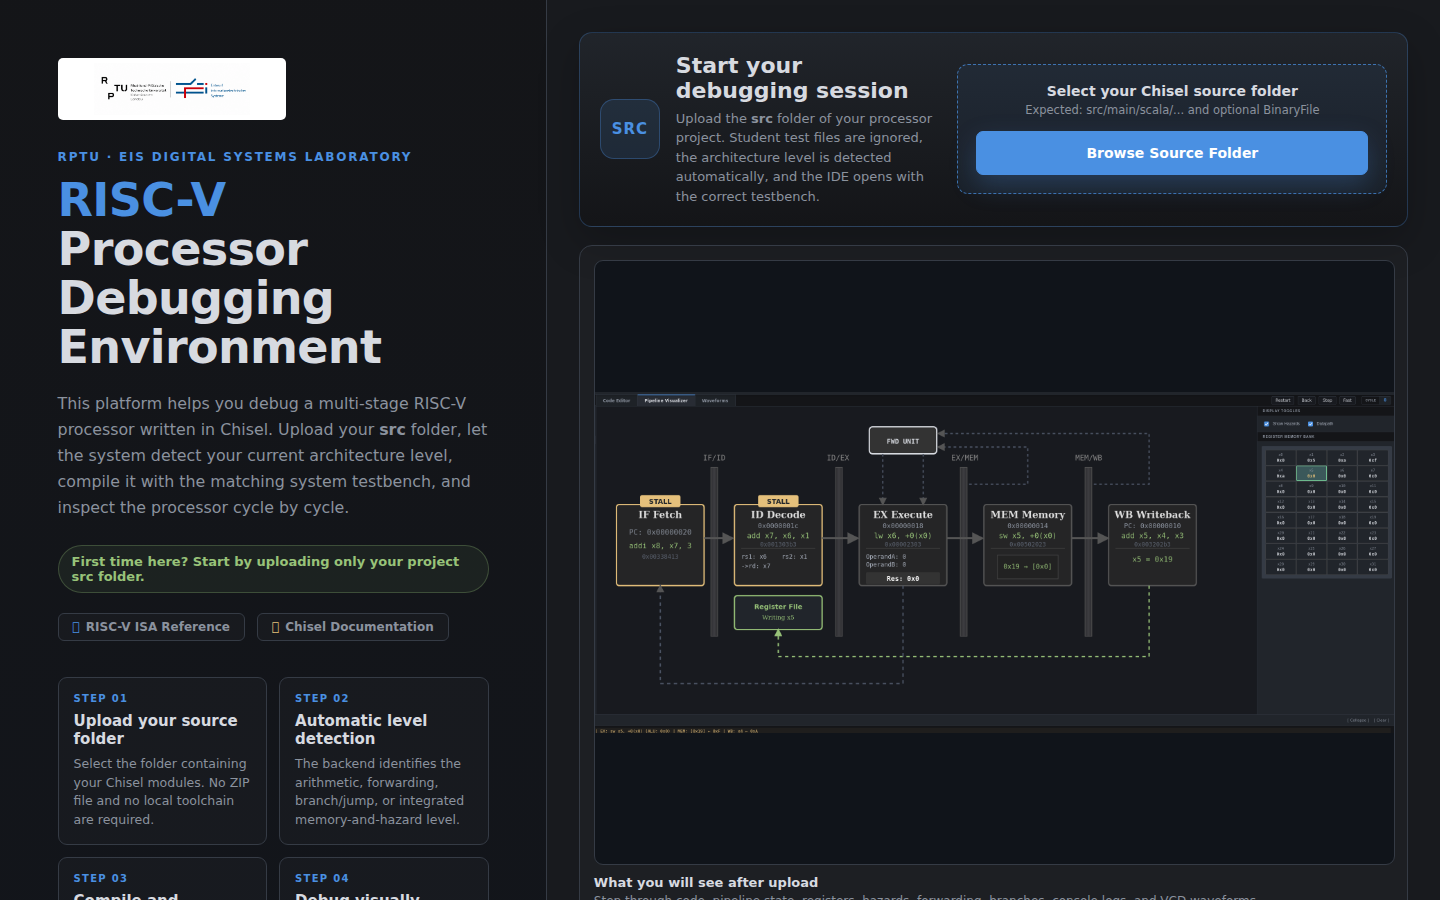
\includegraphics[width=0.93\textwidth]{landing_interface.png}
  \caption{First-use interface. The student selects the project \texttt{src} directory and the service detects the course level before compilation.}
  \label{fig:landing}
\end{figure}

\section{Installation and first startup}\label{sec:installation}

\subsection{Prerequisites and assisted setup}

The host requires Python~3 with virtual-environment support, a compatible Java Development Kit, SBT, and internet access for initial dependency resolution. JDK~17 and SBT~1.9.7 were used for final validation. The repository is obtained and prepared with Listing~\ref{lst:quick-install}.

\begin{lstlisting}[style=terminal,caption={Clone, setup, and startup commands.},label={lst:quick-install}]
git clone https://github.com/RPTU-EIS/RISCV-pipeline-vizualizer.git
cd RISCV-pipeline-vizualizer
./scripts/setup.sh
./scripts/run.sh
\end{lstlisting}

If GitHub SSH access is already configured, the equivalent clone command is \texttt{git clone git@github.com:RPTU-EIS/RISCV-pipeline-vizualizer.git}.

The setup script determines the repository root from its own location, creates or reuses \texttt{.venv}, and installs the pinned packages from \texttt{requirements.txt}. It then checks Java and SBT and reports whether the complete simulation environment is ready. Missing prerequisites produce a nonzero exit status and an installation command or official download link; the script does not silently download a JDK or SBT. The first SBT dependency resolution requires an internet connection and can take appreciably longer than later starts. Running \texttt{sbt --batch update} once is therefore recommended before a class~\cite{sbt-docs}.

The run script activates the repository-local environment and starts the service independently of the caller's current directory. The terminal prints the browser address, normally \url{http://127.0.0.1:8080}. Both scripts were tested when invoked from outside the repository.

\subsection{Manual setup and first upload}

If the helper cannot be used, the Python portion can be prepared manually:

\begin{lstlisting}[style=terminal]
python3 -m venv .venv
.venv/bin/python -m pip install --upgrade pip
.venv/bin/python -m pip install -r requirements.txt
sbt --batch update
.venv/bin/python web_demo.py
\end{lstlisting}

After opening the printed local address, the user selects the \texttt{src} directory of a course project, not the repository root. The upload is reviewed before compilation. A \texttt{BinaryFile} is a hexadecimal machine-code program with one 32-bit instruction word per line; it is not assembly-language source. The interface can use the system BinaryFile for the detected level or a custom BinaryFile supplied by the student.

\begin{table}[tb]
\centering
\caption{Concise startup troubleshooting guide.}
\label{tab:troubleshooting}
\small
\begin{tabularx}{\textwidth}{@{}p{0.22\textwidth}YY@{}}
\toprule
Symptom & Likely cause & Action \\
\midrule
Python or virtual environment fails & Python or the \texttt{venv} package is absent & Follow the command printed by the setup script, then rerun it. \\
Java or SBT check fails & Simulation prerequisite is absent from \texttt{PATH} & Install JDK~17 and SBT using the displayed official guidance. \\
First compile appears slow & SBT is resolving Scala and Chisel dependencies & Keep internet access available and allow the first run to finish. \\
Browser does not open & Desktop integration is unavailable & Open the address printed in the terminal manually. \\
Scala compilation fails & Submitted sources do not compile against the scaffold & Read the browser log; local session paths appear as \texttt{[WORKSPACE]}. \\
\bottomrule
\end{tabularx}
\end{table}

\section{Use in teaching}\label{sec:teaching}

The instructor prepares the computer, performs the first dependency download, and starts the local service. They also provide or approve the source projects and system BinaryFiles used in an exercise. Because compilation executes uploaded Scala/Chisel, the validated setting is a trusted local laboratory; exposing the service to untrusted users is outside its present scope.

The student selects the relevant \texttt{src} directory. The browser sends accepted source files to the service, which detects the level from project structure and content. The student reviews the detected level and the files shown in the editor, then chooses the system or custom BinaryFile and compiles. The custom program format is deliberately direct: one eight-digit hexadecimal instruction word per line, with no labels, mnemonics, or assembler directives.

After compilation, the student starts the simulation and moves forward one cycle at a time. The main view shows which instruction is in IF, ID, EX, MEM, and WB. The register panel shows register values, and the terminal shows compile and cycle messages. Highlights show forwarding, stalls, and flushes. Students can return to an earlier saved cycle without running the processor again, and can open the generated VCD waveform in Surfer. Edited source files can also be exported.

This sequence supports several teaching patterns. An instructor can ask students to predict the next pipeline state before stepping; students can compare a forwarding implementation with the register values it produces; and a branch exercise can relate the EX-stage decision to the younger instructions being flushed. The visualizer does not replace normal tests. It provides a focused explanation of a failing or surprising cycle so that a student can return to the Chisel implementation with a specific hypothesis.

\section{System architecture}\label{sec:architecture}

The system has three main parts, summarized in Figure~\ref{fig:architecture}. The browser lets the student upload files, edit code, step through cycles, and view the pipeline, registers, log, and waveform. The Python web service receives requests and sends updates back to the correct browser window. The simulation part uses SBT, Chisel, chiseltest, and \texttt{LivePipelineTest.scala} to build and run the processor. Chisel is a hardware-design language written in Scala~\cite{chisel-docs}, and chiseltest provides the clocked tests used here~\cite{chiseltest}.

\begin{figure}[tb]
  \centering
  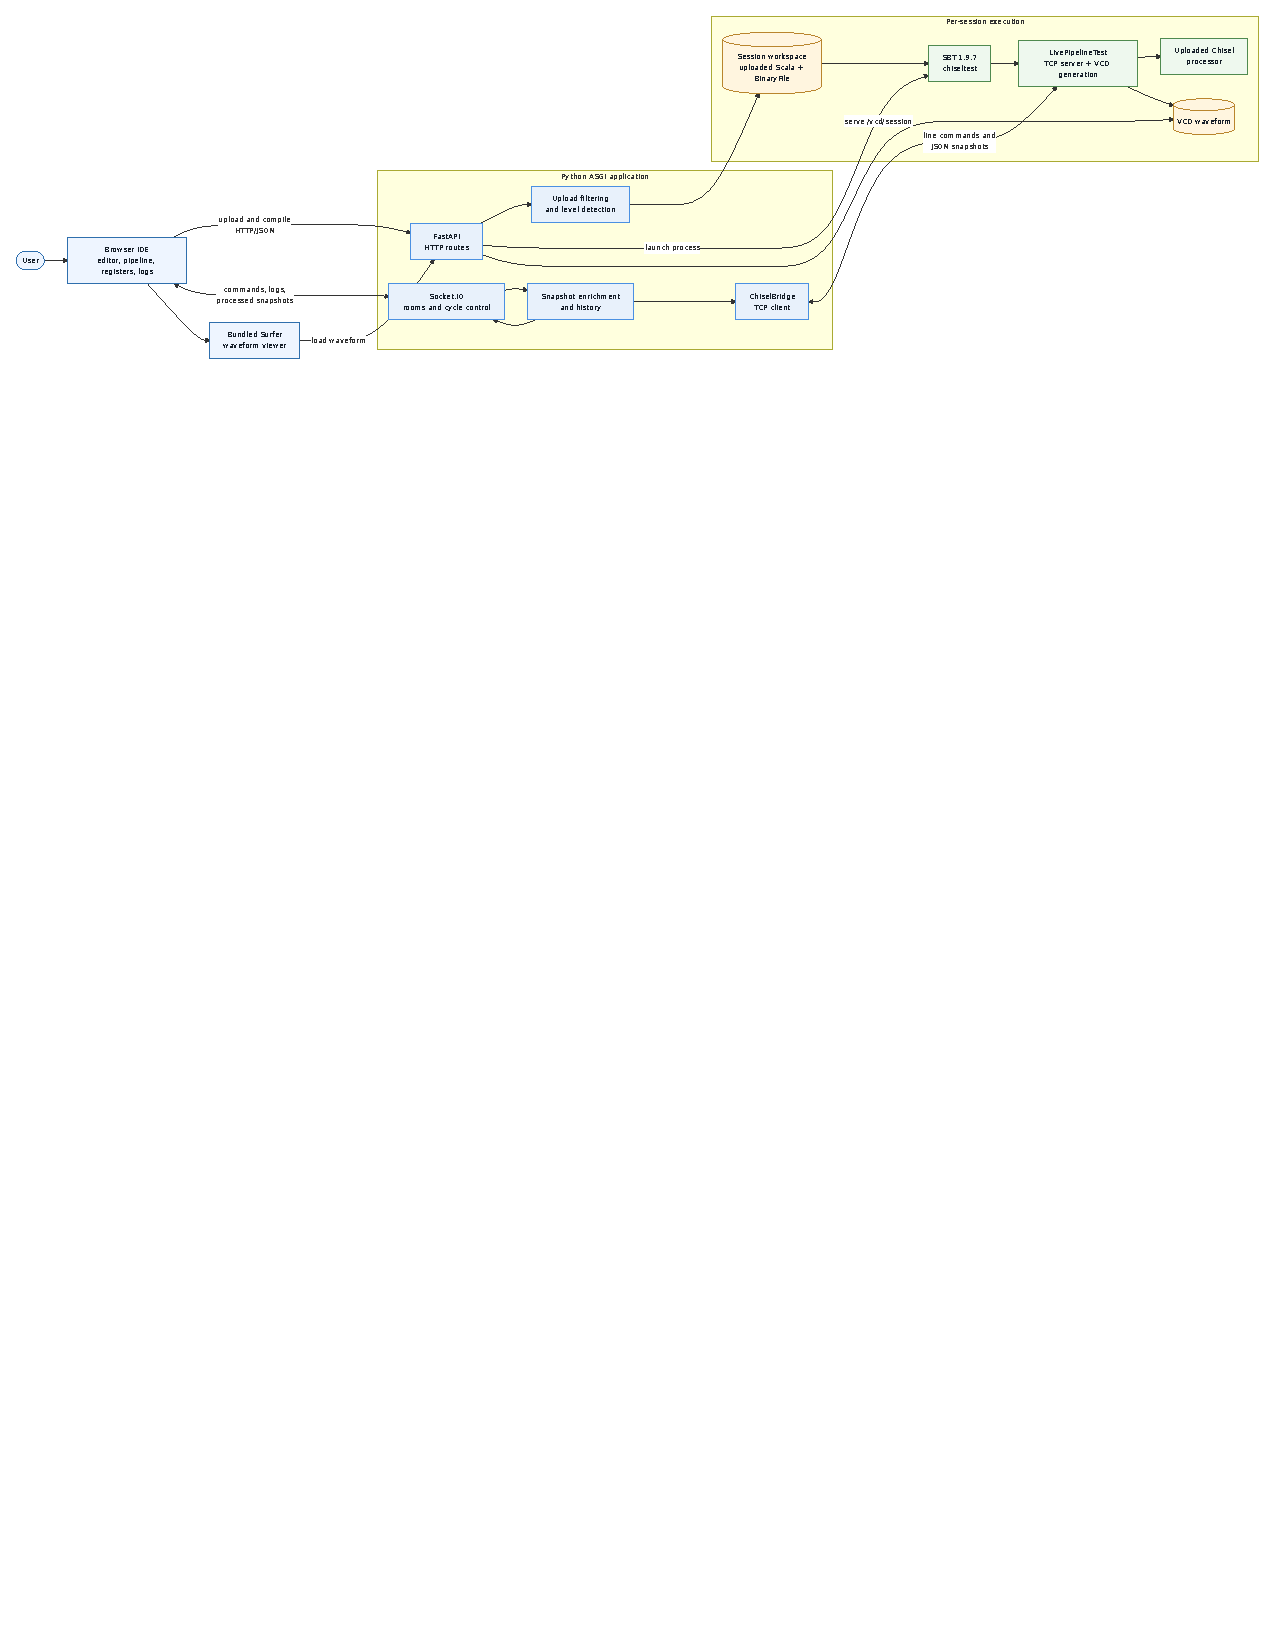
\includegraphics[width=\textwidth,trim=10bp 386bp 10bp 10bp,clip]{system_architecture.pdf}
  \caption{System architecture. HTTP handles upload, compilation, static content, and VCD delivery; Socket.IO carries cycle commands and updates; a per-session testbench process runs the uploaded processor.}
  \label{fig:architecture}
\end{figure}

\texttt{web\_demo.py} starts the local web server and prints its address. \texttt{web\_visualizer/server.py} receives uploads, detects the course level, prepares a temporary work folder, starts SBT, and stores the cycles already shown. \texttt{web\_visualizer/bridge.py} is the small connection between the Python service and the Scala simulation.

For compilation, the service copies a prepared template into a temporary work folder, adds the accepted student Scala files, and writes the chosen BinaryFile where the test expects it. SBT starts \texttt{LivePipelineTest}, which builds the processor and opens a local connection for this session. Python sends simple commands such as \texttt{step}; the testbench sends back a snapshot of the processor state. This keeps the browser separate from the details of the simulator.

Each browser window has its own session. When the user chooses \texttt{init} or \texttt{step}, the request goes to the simulation and the returned state is saved. The browser then updates the pipeline drawing and register table. The testbench creates the VCD waveform file, and the service gives Surfer access to the file for the same session~\cite{surfer}.

\section{Five-stage pipeline visualization}\label{sec:pipeline}

The visual model uses the usual IF, ID, EX, MEM, and WB stages shown in Figure~\ref{fig:pipeline}. IF fetches the next instruction. ID reads and decodes it. EX performs arithmetic, checks branches, or calculates an address. MEM accesses data memory when needed. WB writes a result back to the register file. Registers between the stages allow several instructions to be processed at the same time.

\begin{figure}[tb]
  \centering
  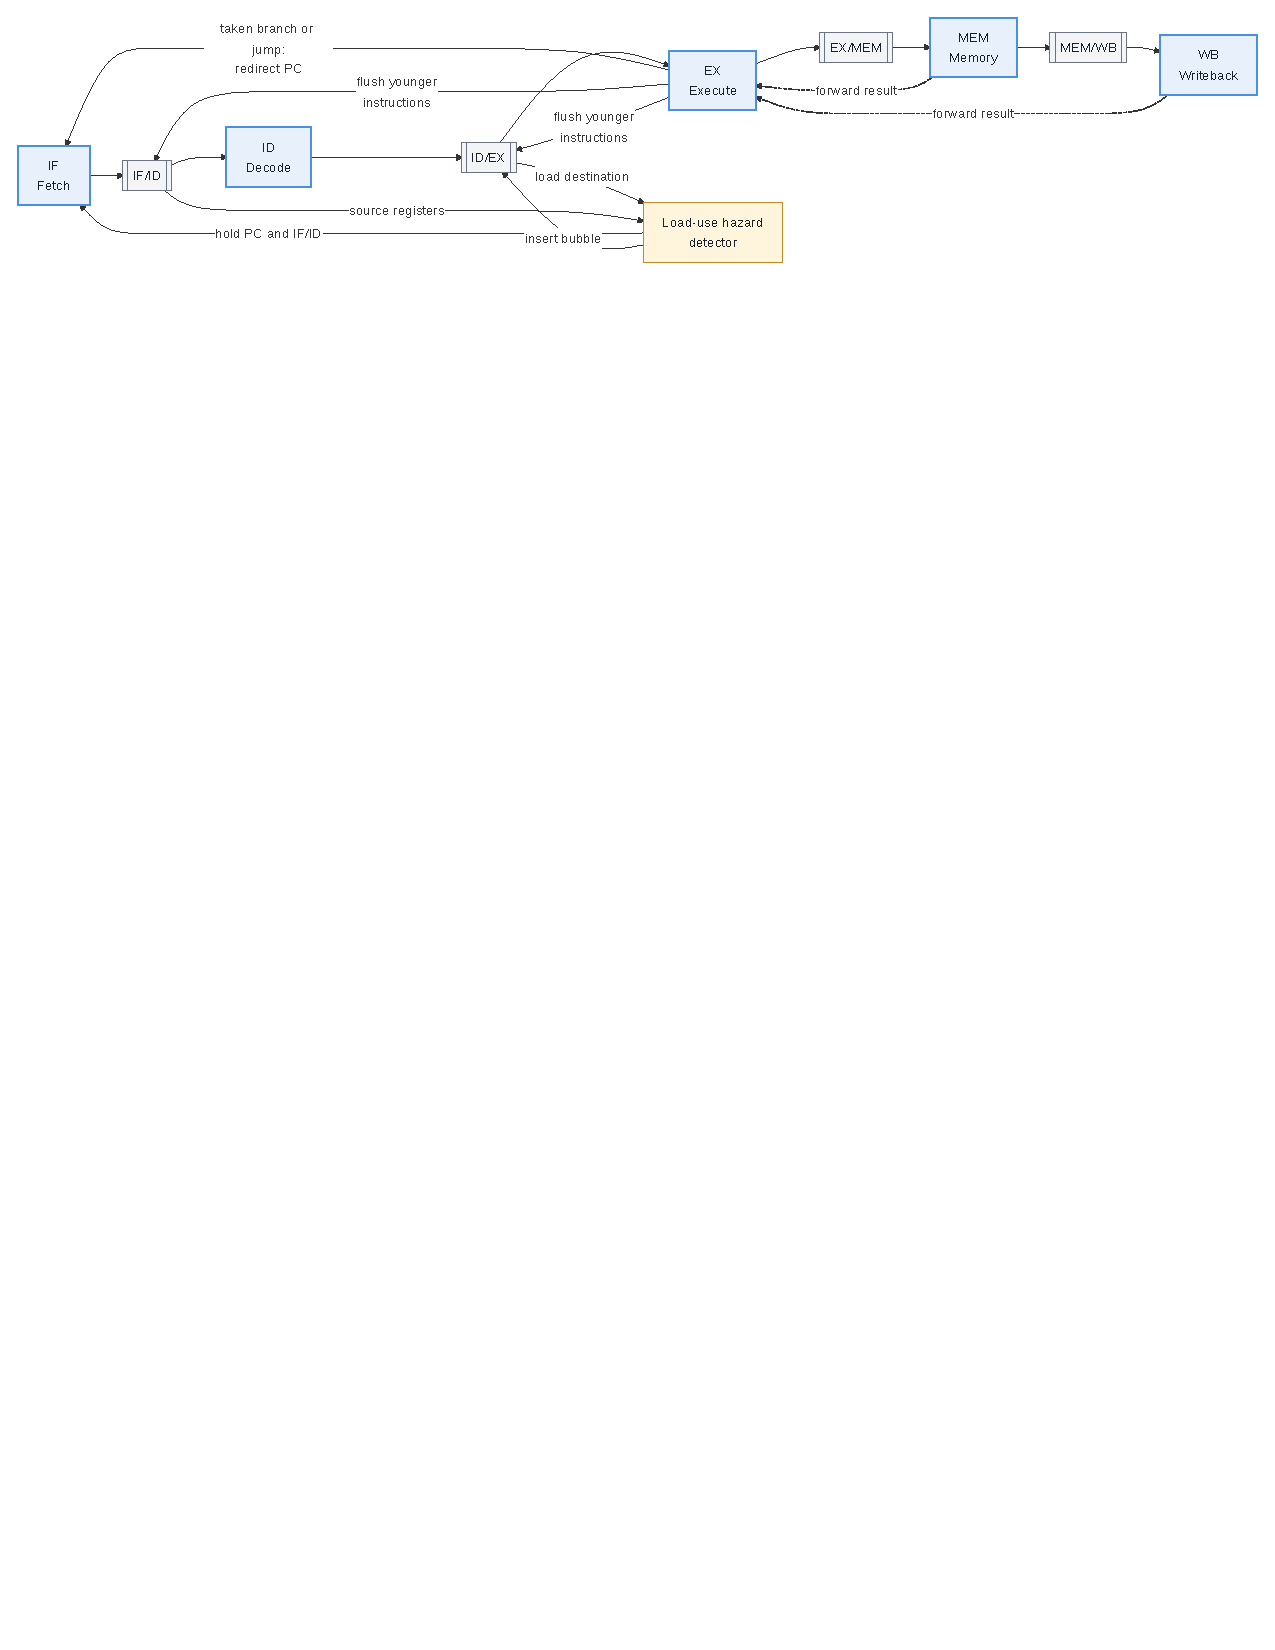
\includegraphics[width=\textwidth,trim=8bp 630bp 8bp 8bp,clip]{five_stage_pipeline.pdf}
  \caption{Simplified five-stage datapath and hazard paths. Dashed paths represent forwarding; control and load-use decisions can redirect, hold, flush, or inject a bubble.}
  \label{fig:pipeline}
\end{figure}

The display turns each saved processor state into this simpler picture. Each stage box shows its instruction and program counter. Hazard highlights show the important control signals for that cycle. The picture does not include every Chisel signal. Instead, it shows useful relationships, such as a value from MEM being used by EX.

An instruction sometimes needs a value that an earlier instruction has not written back yet. If that value is already available in a later stage, forwarding sends it directly to EX instead of waiting for the register file. The Level~2 view shows which forwarding path is active. A load-use dependency is different: a load returns its data too late for the next instruction. The processor must pause the program counter and IF/ID stage for one cycle and insert an empty operation (a bubble).

Branches and jumps can fetch instructions from the wrong path before the decision is known. In the demonstrated Level~3 design, that decision is made in EX. When a branch is taken, the processor fetches from the target address and removes the younger instructions from the old path. The interface shows the target and the flush together. These descriptions apply to the supplied course processors, not to every possible RISC-V design.

\section{Compilation and simulation workflow}\label{sec:workflow}

The sequence is shown in Figure~\ref{fig:sequence}. Uploading and compilation use normal web requests. Interactive stepping uses Socket.IO so that the server can send logs and processor updates back to the correct browser session. The server detects the project level itself; the browser does not choose it during compilation.

\begin{figure}[tb]
  \centering
  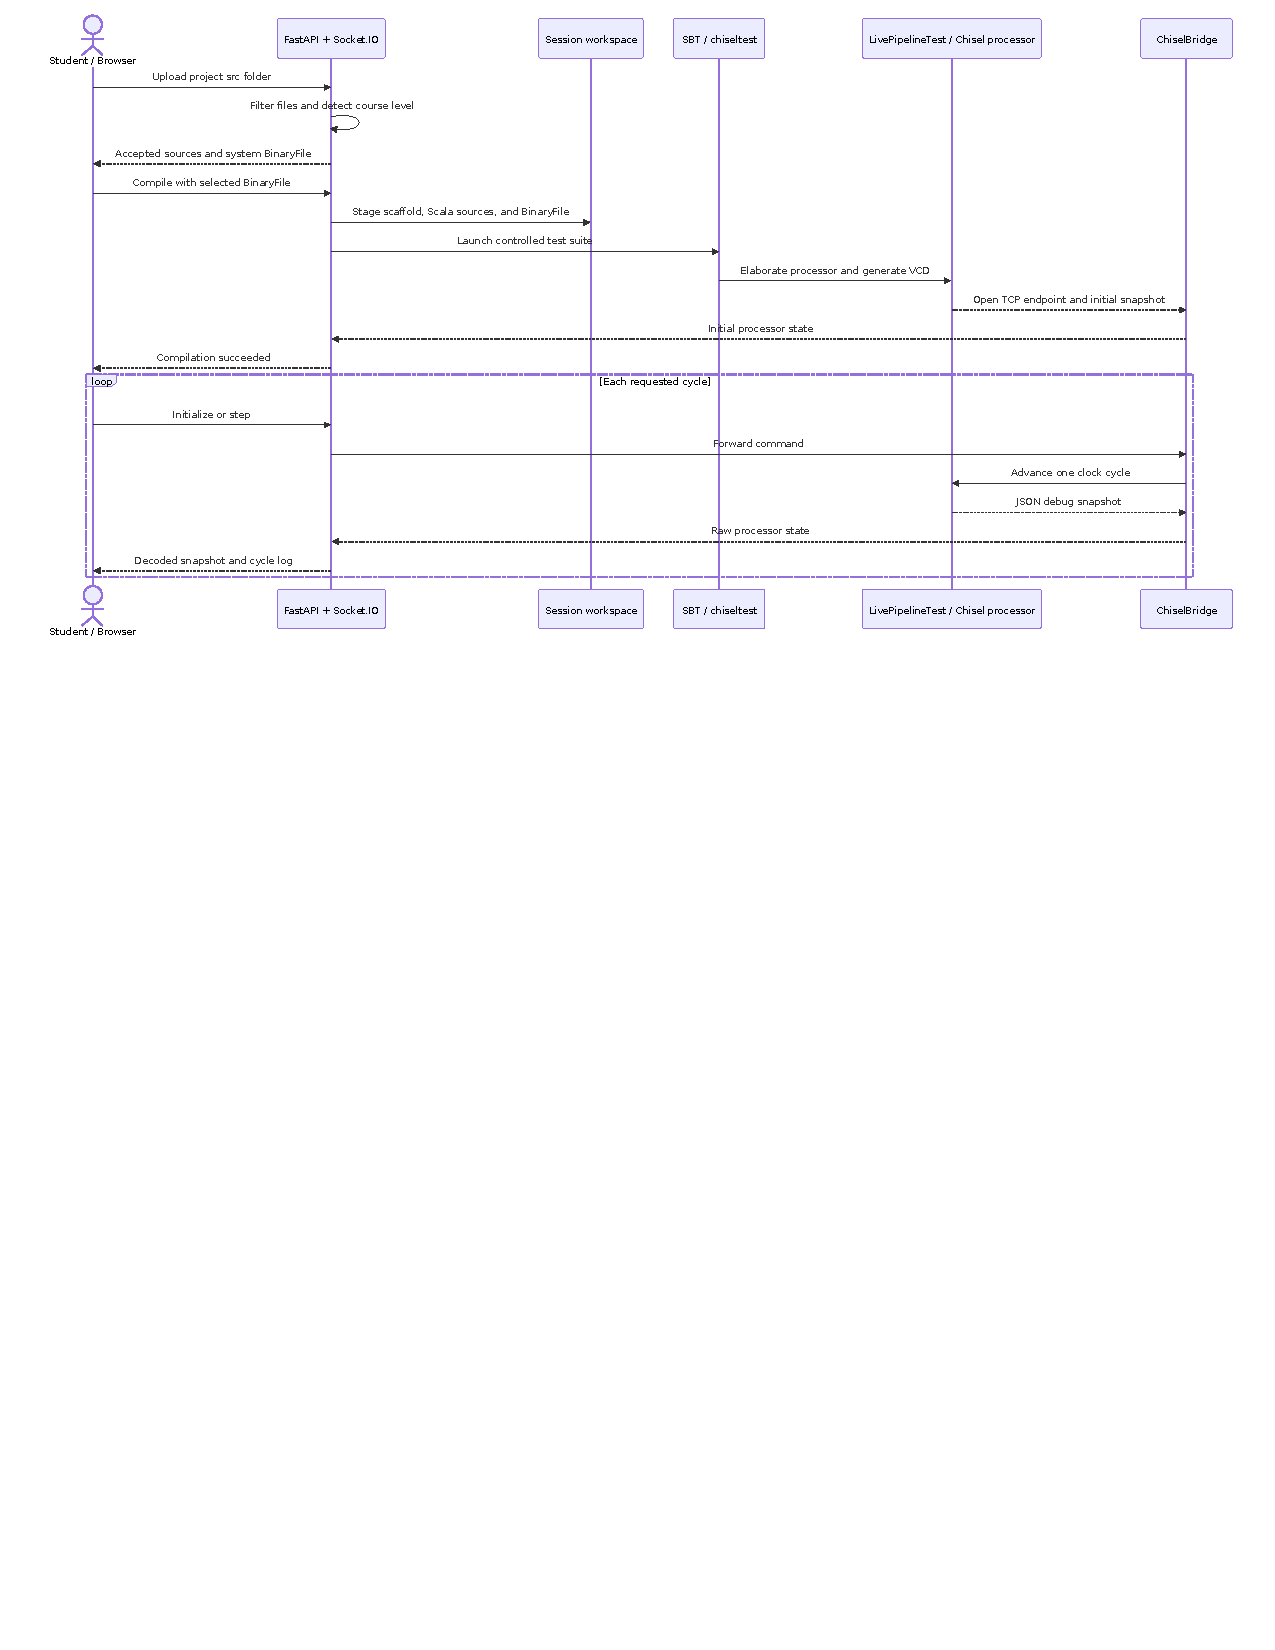
\includegraphics[width=\textwidth,trim=24bp 487bp 20bp 7bp,clip]{execution_sequence.pdf}
  \caption{Execution sequence from source selection to a rendered cycle. The controlled testbench advances the clock and returns one JSON snapshot for each step command.}
  \label{fig:sequence}
\end{figure}

During upload, the service accepts the files needed for the exercise and ignores unsafe or unrelated paths. Messages shown in the browser use \texttt{[WORKSPACE]} instead of a student's local computer path. If Scala compilation fails, the browser still receives the useful explanation and SBT output.

Before interactive stepping, the testbench runs once to create a VCD waveform file. Surfer can open this file to show signal timing alongside the pipeline view, as shown in Figure~\ref{fig:waveform}. The testbench then resets the processor and sends the first state. Every \texttt{step} command advances one clock cycle and returns one snapshot of the debug values. Python turns instruction words into readable text, saves the snapshot, and updates the browser. From the student's point of view, one accepted step means one displayed cycle.

\begin{center}
  \centering
  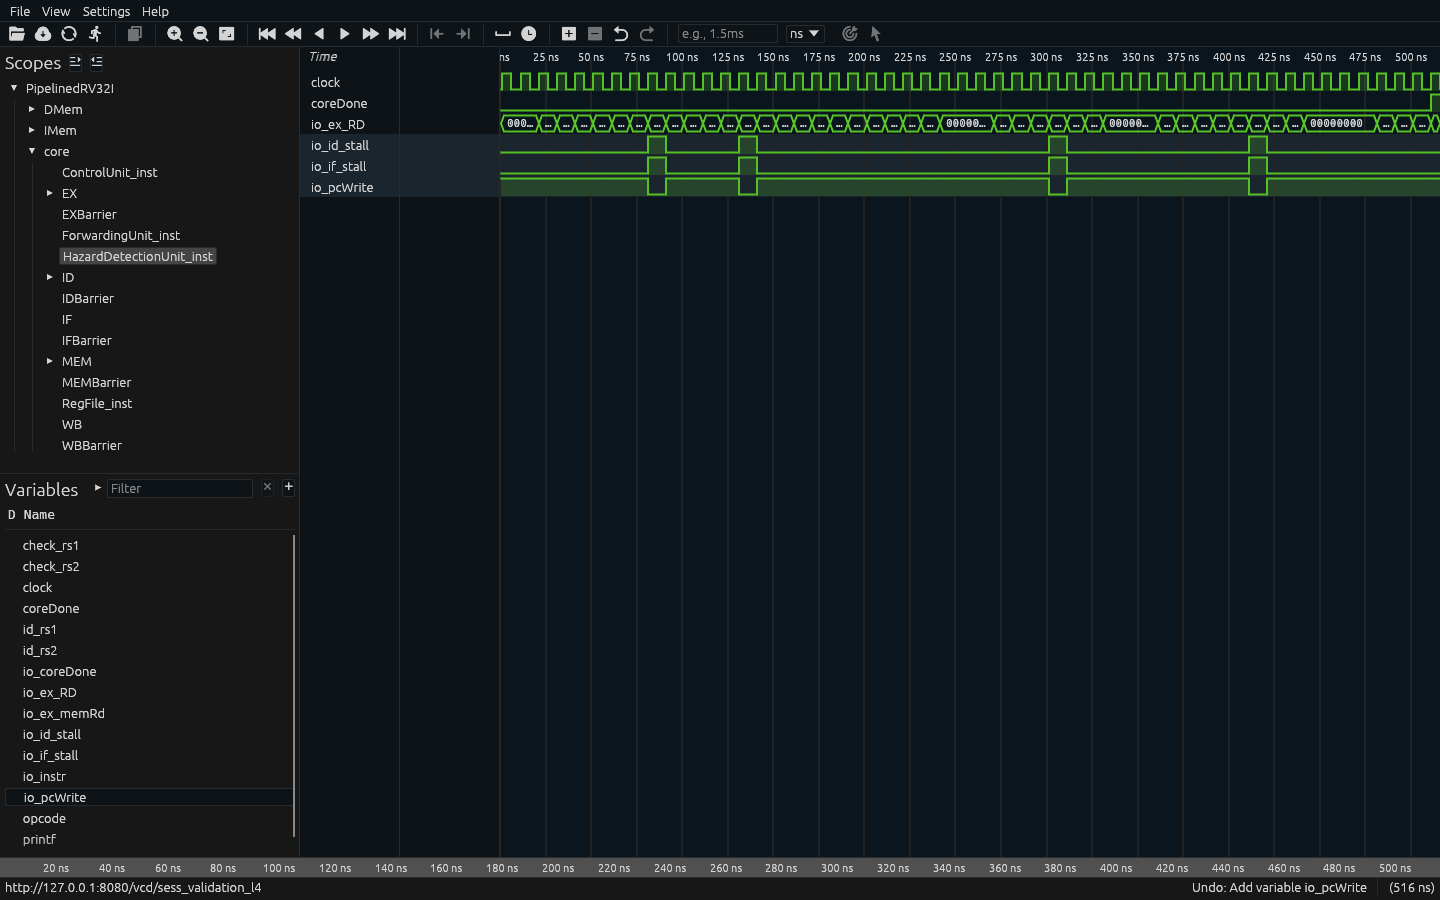
\includegraphics[width=0.96\textwidth]{waveform_view.png}
  \captionof{figure}{Generated Level~4 waveform displayed in the bundled Surfer viewer. The selected clock and processor debug signals complement the cycle-level pipeline representation.}
  \label{fig:waveform}
\end{center}

The supplied simulation structure and VCD limits are preserved. Forwarding, stalls, branches, memory behavior, and instruction coverage remain properties of the uploaded course core and controlled infrastructure, not of the web interface.

\section{Demonstrated pipeline behavior}\label{sec:behavior}

The four supplied reference levels were tested through the complete upload, compilation, and simulation workflow; their representative programs completed at cycles 12, 12, 15, and 51 respectively. Level~1 demonstrated the basic arithmetic pipeline, Level~2 forwarding without stalls or flushes, Level~3 a taken branch and removal of younger instructions, and Level~4 forwarding, load-use holds, control-flow recovery, and memory behavior. Because the programs differ, their run lengths are not a performance comparison.

Figure~\ref{fig:hazards} compares Level~2 forwarding at cycle~3, a Level~3 taken-branch flush at cycle~7, and a Level~4 load-use hold of the program counter and IF/ID at cycle~41.

\clearpage
\newgeometry{left=1.5cm,right=1.5cm,top=2cm,bottom=2cm}
\begin{figure}[p]
  \centering
  \begin{subfigure}[t]{0.86\textwidth}
    \centering
    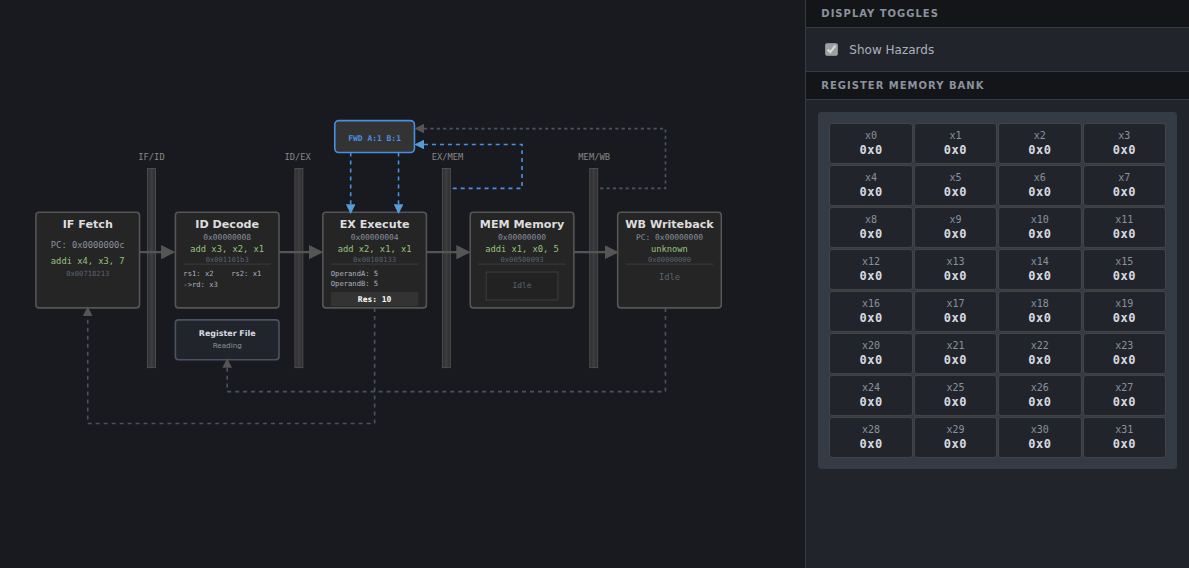
\includegraphics[width=\linewidth]{level2_forwarding_cycle_03.png}
    \caption{Level~2 forwarding, cycle~3.}
  \end{subfigure}\par\smallskip
  \begin{subfigure}[t]{0.86\textwidth}
    \centering
    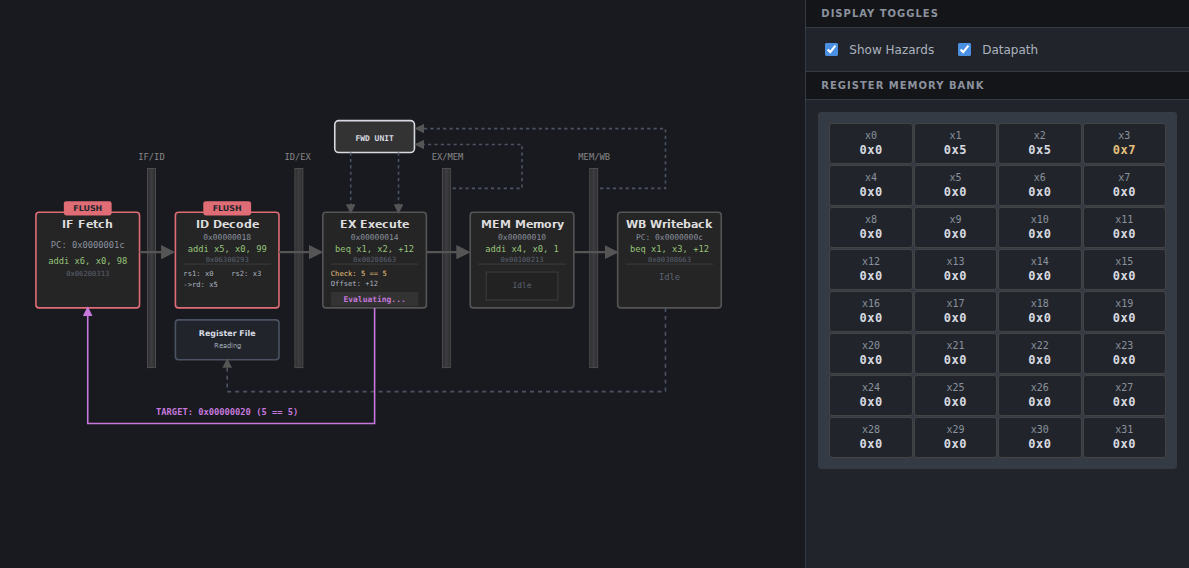
\includegraphics[width=\linewidth]{level3_branch_flush_cycle_07.png}
    \caption{Level~3 taken branch and flush, cycle~7.}
  \end{subfigure}\par\smallskip
  \begin{subfigure}[t]{0.86\textwidth}
    \centering
    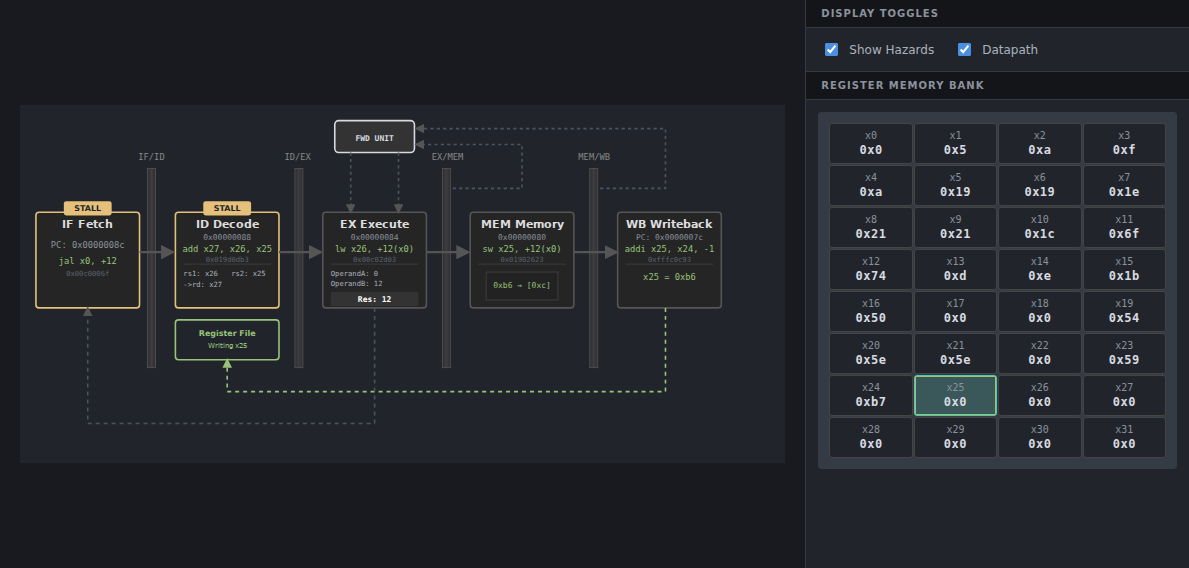
\includegraphics[width=\linewidth]{level4_load_use_stall_cycle_41.png}
    \caption{Level~4 load-use stall, cycle~41.}
  \end{subfigure}
  \caption{Representative pipeline-hazard responses: forwarding in Level~2, branch flushing in Level~3, and a load-use stall in Level~4.}
  \label{fig:hazards}
\end{figure}
\clearpage
\restoregeometry

Together, the panels show that the same stage view can explain three distinct responses to dependency and control-flow conditions. Forwarding changes the EX operand source without interrupting instruction issue. A taken branch redirects fetch and invalidates younger fall-through instructions. The load-use case instead holds the front of the pipeline for one cycle because the required memory value is not yet available. The register panel and highlighted paths connect each control decision to the architectural state observed by the student.

\section{Maintenance and future development}\label{sec:maintenance}

The repository keeps the startup code, browser code, simulation code, and course material in separate places, so most changes have a clear starting point. Appendix~\ref{app:implementation-map} lists the main files. The most important connection to understand is between the Python service and the Scala testbench.

Changes between Python and Scala need care. For example, renaming a JSON field means changing the testbench, Python bridge, saved history, and browser code. Showing a new pipeline signal usually needs a Chisel debug output, a value in the snapshot, and a matching element in the browser. Level detection should be tested with representative project folders and should remain a server decision.

Future work should match the intended local teaching use. The browser libraries could be stored locally for optional offline use. Better session cleanup would help when the tool runs for a long time or serves more than one user. A public network version would need login controls, safer uploads, and stronger isolation before it could be used safely. More automated browser and processor tests would also make maintenance easier. Any correction to signed \texttt{SRA} or \texttt{SLT} behaviour should first be checked with processor tests and approved by the supervisor.

\section{Conclusion}\label{sec:conclusion}

The RISC-V Pipeline Visualizer helps students inspect a processor one clock cycle at a time without taking over the processor design. The browser connects source files and machine-code input with pipeline stages, registers, hazards, logs, and VCD waveforms. The Chisel testbench still performs the actual simulation. The setup scripts and documentation make the project easier to hand over, and the four course levels use the same descriptions in the interface and report. In its intended trusted local setting, the tool supports lab demonstrations and cycle-by-cycle debugging. Future work should improve reliability and test coverage before changing processor behaviour or exposing the tool more widely.

\bibliographystyle{plainnat}
\bibliography{references}
\addcontentsline{toc}{section}{References}

\clearpage
\appendix
\section{Implementation map}\label{app:implementation-map}

\begin{center}
\centering
\captionof{table}{Principal implementation and maintenance files.}
\label{tab:implementation-map}
\footnotesize
\begin{tabularx}{\textwidth}{@{}>{\raggedright\arraybackslash}p{0.43\textwidth}Y@{}}
\toprule
Path & Responsibility \\
\midrule
\path{web_demo.py} & Local entry point and browser-address reporting. \\
\path{web_visualizer/server.py} & HTTP/Socket.IO API, filtering, detection, staging, process launch, history, and VCD delivery. \\
\path{web_visualizer/bridge.py} & TCP command and snapshot exchange with the Scala testbench. \\
\path{web_visualizer/templates/index.html} & Interface, editor, controls, rendering logic, and student terminology. \\
\path{web_visualizer/static/pipeline.svg} & Visual structure and element identifiers used by the renderer. \\
\path{infrastructure_template/src/test/scala/LivePipelineTest.scala} & Controlled headless and interactive chiseltest behavior, snapshot schema, and VCD production. \\
\path{course_material/} & Reference sources for the staged course levels. \\
\path{infrastructure_template/system_tests/} & Level-specific hexadecimal BinaryFiles and test inputs. \\
\bottomrule
\end{tabularx}
\end{center}

\section{Scope of validation}

Evaluation of the complete workflow used the supplied system BinaryFiles and completed all four detected course levels. The evaluation covered shell and Python syntax, setup and startup from outside the repository, upload and detection, compilation without a client-supplied level, interactive stepping, pipeline and register rendering, hazard overlays, sanitized browser messages, VCD delivery, and Surfer loading. Processor ISA conformance beyond the supplied programs and existing Scala tests was not re-certified. Multi-user load, malicious uploads, and public deployment were not tested because they are outside the trusted local teaching scope.

\end{document}
